\chapter{Project outline}
It has previously been found that there is a good relationship between the intake of digestible organic matter and gain in cattle \cite{Lippke1980}. Extending this, we postulate that there is a correlation between the amount of chewing events (ie individual chews or bites) and the amount of intake. Therefore, rather than trying to exactly quantify the intake of pasture in livestock the project will aim to quantify the amount of chewing events. 

The postulated correlation between chewing events and amount of intake can be experimentally confirmed. By weighing groups of livestock individually before and after a trial a relationship between the amount of time the animal spent feeding and the weight it gained can be confirmed. 

The main goal of the project is therefore automating the quantification of the amount of chewing events in individual livestock. As previously stated, this information can assist in the economic goals of livestock management by creating selective breeding opportunities. 

\section{Previous work}

Currently, CSIRO have performed experiments where sensor nodes are deployed on the eartags of cattle. Sensor nodes are capable of collecting sensor data, processing and communicating with other sensor nodes over a network. A collection of sensor nodes communicating wirelessly form a Wireless Sensor Network (WSN). The sensor node eartag platform is based on the 16 bit CC430F5137 microcontroller unit and has a range of sensors including audio, GPS, accelerometer, magnetometer and gyroscope. A photo of the eartag is shown in figure \ref{eartag} and a photo of the eartag attached to a cow is shown in figure \ref{cow}.


\begin{figure}[H]
\centering
\begin{minipage}{.5\textwidth}
  \centering
  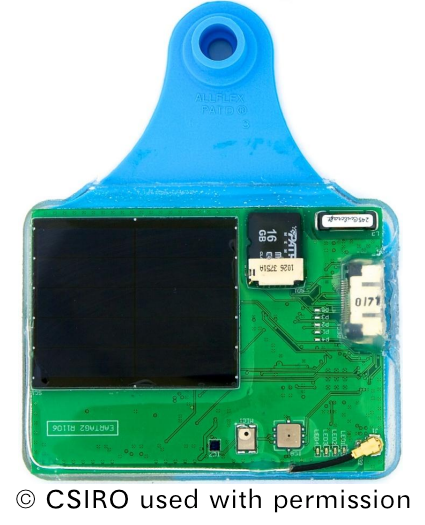
\includegraphics[width=0.4\textwidth]{images/eartag.png}
  \caption{Eartag}
  \label{eartag}
\end{minipage}%
\begin{minipage}{.5\textwidth}
  \centering
  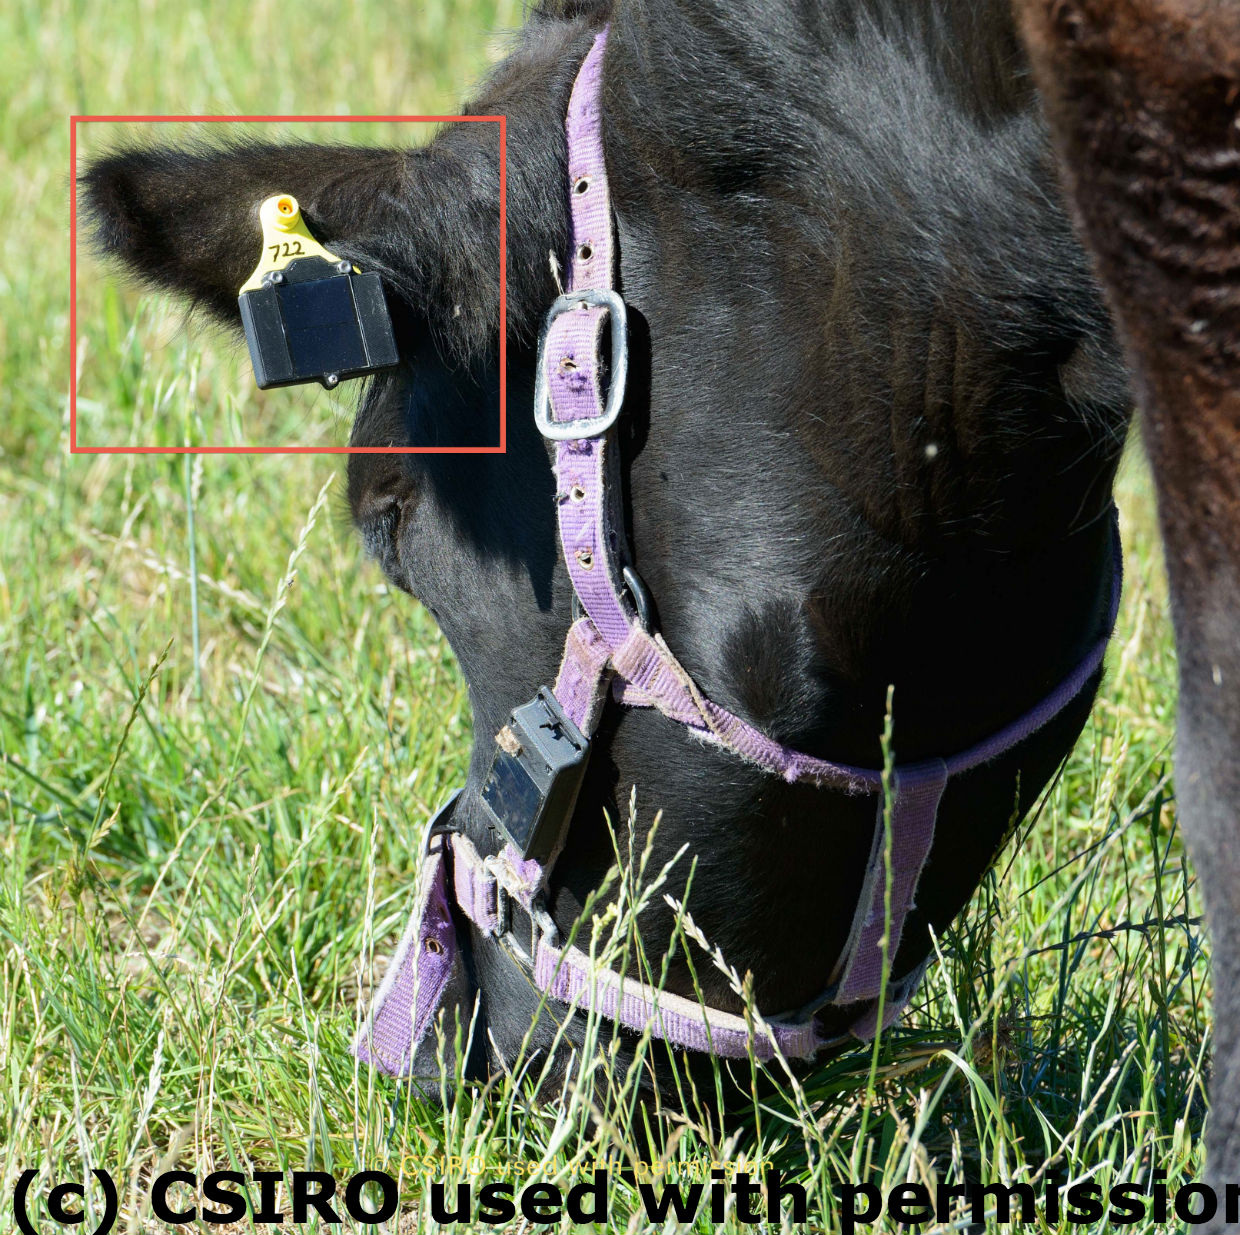
\includegraphics[width=.5\textwidth]{images/cow.jpg}
  \caption{Cow wearing eartag}
  \label{cow}
\end{minipage}
\end{figure}


The WSN platform has been used for animal behaviour classification in the past as seen in section 2.1. It is ideal for the task of real-time classification as sensor nodes are small, low cost, able to communicate wirelessly and run at low power. The eartag platform is powered by a battery and solar panel so that it is possible to run for extended periods. In addition, the sensors nodes are capable of processing so it would be possible to run a classification algorithm on a node. 

CSIRO have performed experiments in a variety of conditions where time-stamped data from sensor nodes attached to cattle is recorded while the cattle behaviour is recorded with video. In this way, data from the eartag can be matched with particular behaviours of the cattle. A classification algorithm can then be designed using this data.

\section{Goals}

Using the data recorded in the experiments outlined in section 3.1, the main goal of this project is to develop a classifier that can run on the sensor node eartag platform and quantify the amount of time individual cows spend feeding. Although the result of this work will be specific to cattle, it is envisioned that the technique will be transferable to other species of livestock. 

In designing a classifier to measure the amount of time individual cattle spend feeding, it may also be advantageous to classify other simple behaviour modes of the cattle. For example, measuring whether a cow is currently travelling is helpful in estimating whether it is feeding, as a cow is more likely to eat while stationary. These extra behavioural modes of the cattle can also assist in livestock management, for example a sick or injured cow can be identified from the fact it has not recently travelled or is constantly still. 

Though the sensor node eartag platform is inherently low power, it is advantageous to optimise the power usage of any software on the sensor node. In this way, another goal of the project is for the classifier's power usage to be low enough to that it can run for long periods on only the attached battery and solar panel.
